\documentclass[journal]{IEEEtran}
\IEEEoverridecommandlockouts
% The preceding line is only needed to identify funding in the first footnote. If that is unneeded, please comment it out.
\usepackage{cite}
\usepackage{amsmath,amssymb,amsfonts}
\usepackage{algorithmic}
\usepackage{graphicx}
\usepackage{textcomp}
\usepackage{xcolor}
\usepackage{orcidlink}
\usepackage{amsmath}
\def\BibTeX{{\rm B\kern-.05em{\sc i\kern-.025em b}\kern-.08em
    T\kern-.1667em\lower.7ex\hbox{E}\kern-.125emX}}
\begin{document}

\title{Système d’illumination de trottoir nocturne pour piétons \\
{\footnotesize \textsuperscript{*} ELG 4539: Électronique III}
\thanks{Identify applicable funding agency here. If none, delete this.}
}

\author{\IEEEauthorblockN{1\textsuperscript{st} Idriss Amadou Ali}
\IEEEauthorblockA{\textit{Dept de Science NI:3001516551 } \\
\textit{Université d'Ottawa}\\
Ottawa,Ontario \\
iamad056@uottawa.ca \orcidlink{https://orcid.org/0000-0001-8721-3321}\\}
\and
\IEEEauthorblockN{2\textsuperscript{nd} Marc-Antoine Mayer}
\IEEEauthorblockA{\textit{Dept de Génie NI:300052042} \\
\textit{Université d'Ottawa}\\
Ottawa,Ontario \\
mmaye047@uottawa.ca\\
}

}

\maketitle

\begin{abstract}
    Nous avons construits un dispositif capable de différencier les entités 
    sur le trottoir basé sur des capteurs de mouvement infra-rouge et des capteurs de poids, 
    tous reliés à un microcontrôleur Arduino, qui effectuera un CAN sur les signaux analogiques 
    et un Raspberry pi 4 qui effectue une prise de décision basée sur le flux de données reçues.
\end{abstract}

\begin{IEEEkeywords}
Raspberry Pi, Arduino, Capteur de Poids, Capteur Infrarouge, Django
\end{IEEEkeywords}

\section{Introduction}
 Le gouvernement du Québec définit la pollution lumineuse comme toute 
lumière projetée vers le ciel qui obstrue l'observation des étoiles \cite{b1}.
 Cet effet est dû à la projection et la réflexion de la lumière vers le ciel ainsi qu'une surabondance de lumière.
  Ce phénomène représente un manque d'efficacité dans le déploiement de la lumière. D'un point de vue environnementaliste, 
  c'est aussi un gaspillage d'énergie puisque l'énergie lumineuse qui s'échappe vers le ciel ne contribue pas à la tâche voulue d'un lampadaire, 
  qui est par exemple d'illuminer une rue ou un trottoir. \\
   Les capteurs infrarouges pyroélectriques (PIR) comptent parmi la classe de capteurs détecteurs thermiques \cite{b2}. 
  Ces capteurs mesurent la radiation incidente grâce au changement de leur température. Lorsqu'on présente au détecteur un certain matériel absorbant, on peut le configurer pour répondre à une certaine plage de fréquences. 
  Les PIR ont été conçus principalement pour la détection des corps humains, ce qui veut dire que les longueurs d'onde désirées sont de huit à douze micromètres. 

\section{Conception}

\subsection{Conception Matérielle}

Pour le hardware du projet, nous avons décidé de sélectionner deux types de capteurs : le HX711 et le SR-501. Le capteur de tension HX711 est composé d’un Wheatstone bridge, ce circuit utilise 4 résistances arrangées comme dans la figure ci-dessous.
Le voltage de sortie mesurée varie selon la tension mécanique appliquée sur le membre du capteur. Il suffit par la suite qu’à calibrer ce voltage de sortie à l’aide un poids ou une force connue. 
Le capteur a une limite de poids de 20 kilogrammes, mais dans le cas des simulations pour ce projet, ce n’est pas un problème. 

\begin{figure}[htbp]
    \centerline{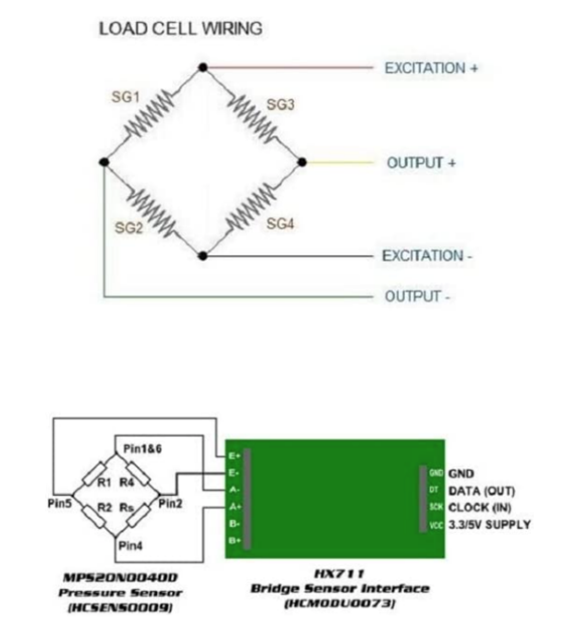
\includegraphics{hardware1.png}}
    \caption{Capteur de Poids HX711.\cite{b3}}
    \label{fig1}
\end{figure} 

Quant au capteurs SR-501, ils fonctionnent en détectant la radiation infra-rouge et en donnant une valeur de sorite binaire, soit 0 ou 1, dépendamment du rapport entre la radiation détectée et un certain seuil. Ces capteurs ont une limitation sur leur temps d’activation. 
Lorsque la sortie d’un capteur passe de 1 à 0, elle sera prise en mode LOW pour 2 secondes. 
Cela veut dire que la sortie du capteur sera fixe à 0 pour deux secondes peu importe la radiation mesurée. Ceci prouve être une contrainte pour la conception des cas de test.\\

Dans notre cas, nous avons 5 capteurs infrarouges et un capteur de poids. 
Le schéma ci-dessous représente le raccordement des capteurs infrarouges à un Arduino. 
Le logiciel utiliser pour ce schéma ne comprenait pas le capteur HX711 dans sa base de données et l’Arduino Nano non plus. Le HX711 as 4 pins, comme vu dans la figure plus haute, où une pin est pour l’alimentation 5 volts, une autre pour la terre, une troisième pour la pin d’entré digitale du Arduino et la dernière pour l’horloge. 
\cite{b4}

\begin{figure}[htbp]
    \centerline{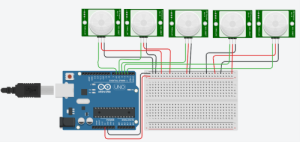
\includegraphics{hardware2.png}}
    \caption{Intégration de capteurs IR Hc-Sr501.\cite{b5}}
    \label{fig2}
\end{figure} 


\subsection{Conception Logicielle}
Afin d'effectuer l'acquisition de données, une synergie entre l'environnement python et C++ arduino est nécessaire. L'état du système sera transféré au rasperry pi qui effectuera
des calculs pour déterminer l'état du système. Cet état sera mis dans un format Json tranférable à un ract dashboard en ligne via protocole https. 

\subsubsection{Code C++}
Ce code sera téléversé sur l'arduino Nano  via l'application platformio IDE. Le microcontrolleur est de type ATnega328P/Pa et cette configuration est nécessaire afin de 
téléverser le code C++ écrtit dans le fichier "main.cpp". Ce fichier prend en charge l'initialisation des capteurs ainsi que la mesure de leurs valeurs et les broadcast continuellement
à une baudrate de  76800 envoi pour réception à baudrate de 19800. le rafraichissement de la boucle principale est 1kHz. 

\begin{figure}[htbp]
    \centerline{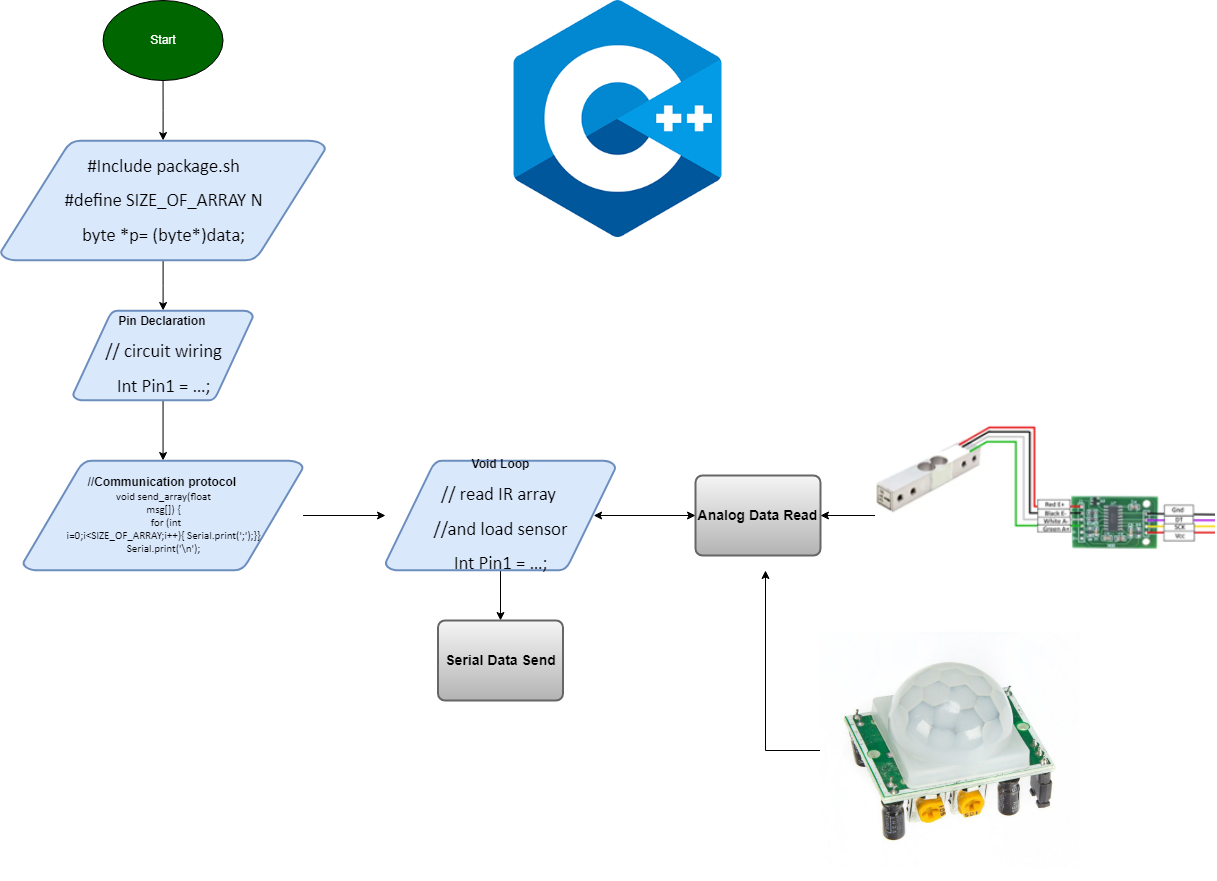
\includegraphics[scale = 0.2]{Trottoir_Flowchart_arduino.drawio.png}}
    \caption{organigramme du Code C++}
    \label{fig3}
\end{figure} 

Pendant l'execution de la boucle principale l'arduino enverra une chaîne de dimension 2 et contenu 8bits , une flottante et un entier. La flottante est le poids capté sur le trottoir et l'entier est un encodage des position
activées de la chaîne de capteur infrarouge. Le plus simple format pour encoder l'entier est l'encodage binaire, cela est fait en multipliant la valeur des capteurs par une la puissande de 2 de leur position, pour 
5 capteurs en commençant à 0:

\begin{equation}\label{eq-1}
    \left\{\begin{aligned}
        V_i \in \{0,1\} \\
        N = \sum_{i=0}^{4}(V_i\cdot 2^i)
    \end{aligned} \right. 
\end{equation}
Cette encodage à l'avantage d'ajouter l'information de la position si la route envisagée est à sens unique et on assume un mouvement dans une direction. L'entier N est la deuxième entrée de la chaîne binare de 
8 bits envoyée par l'arduino.

\subsubsection{Code Python}
Le code python assurera l'intermédiaire entre le dashboard et les capteurs, il décidera l'état du système à afficher gràce à la matrice  d'état suivante:
\begin{figure}[htbp]
    \centerline{\includegraphics[scale = 0.3]{Matrice_décisions.PNG}}
    \caption{Matrice d'états du système}
    \label{fig4}
\end{figure} 

Afin de lire les valeurs des capteurs, le module Serial va détecter l'arduino et se connecter à son port, on tire avantage du parallélisme offert par le language informatique python pour 
définir l'état et l'envoyer à la même vitesse que l'on lit les valeurs des capteurs gràce au module Thread. Une thread va agir en mode daemon(arrière plan) et se terminer lorsque la valeur booléeene définissant
la lecture deviendra 0 ou FALSE.

\begin{figure}[htbp]
    \centerline{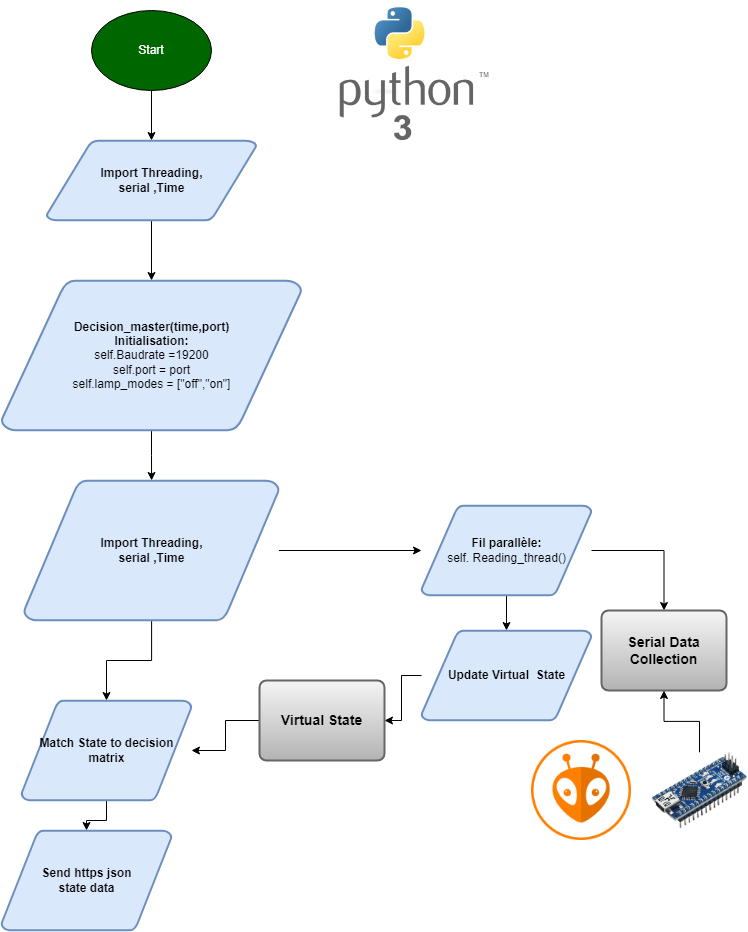
\includegraphics[scale = 0.18]{Trottoir_Flowchart.drawio.png}}
    \caption{Organigramme du code Python}
    \label{fig5}
\end{figure} 

Le code va calculer la vitesse  à partir de la position. Pour décoder la position à partir de N on va utiliser le lgarithme base 2 en combinaison de la fonction partie entière. Les cpateurs infrarouges
sont espacées de d = 15cm et donc la vitesse revient à diviser la différence de position multipliée par d, N étant l'entier lu due l'arduino:

\begin{equation}\label{eq-2}
    \left\{\begin{aligned}
        N = \sum_{i=0}^{4}(V_i\cdot 2^i) \\
        P =  \lfloor{log_2(N)}\rfloor \\
        v = \frac{dP}{dt} = \frac{\Delta P \cdot d}{\Delta t}
    \end{aligned} \right. 
\end{equation}

Le module python time utilisé dans le fil parallèle permet de traquer le temps et effectuer ces mesures.\\
L'état du système est stocké dans un format json prêt à petre envoyé dans une requête https.

\subsubsection{Déploiment Django}

Le backend django permet le déploiment d'un serveur capable de recevoir les requête https, le frontend est un tableau de bord écrits en React javascript.
\begin{figure}[htbp]
    \centerline{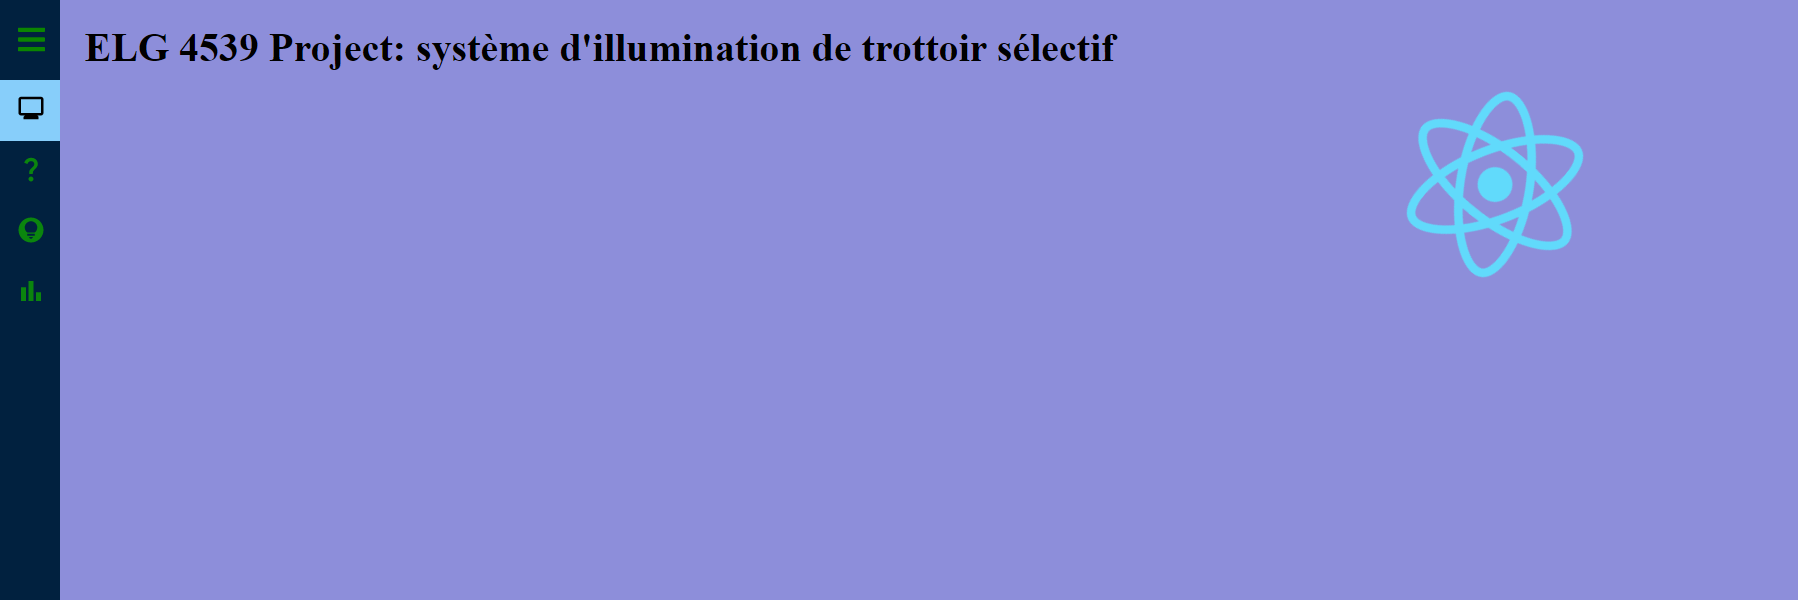
\includegraphics[scale = 0.18]{react_dashboard.PNG}}
    \caption{Tableau de bord react}
    \label{fig6}
\end{figure} 
Le code du projet est disponible sur Github pour consultation \cite{b6}
\\

\section{Mise en Oeuvre}
Afin de compléter le projet le dévellopement Matériel et logiciel à été effectué en parallèle puis joint quand leur dévéloppement fut suffisament accomplis. Le schéma suivante
est donc obtenu:

\begin{figure}[htbp]
    \centerline{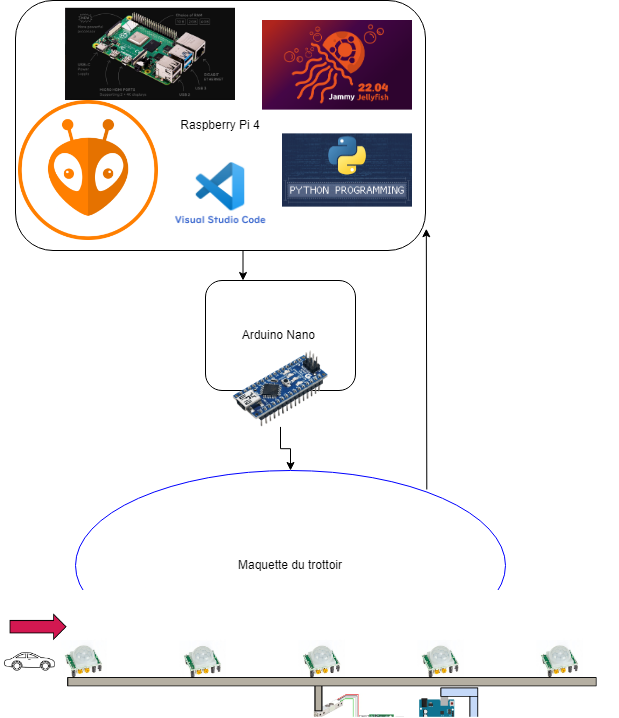
\includegraphics[scale = 0.25]{Trottoir_Diagram.drawio.png}}
    \caption{Schéma du trottoir}
    \label{fig7}
\end{figure} 
Durant la démonstrations des séries de test furent effectués afin de tester les limites de notre design. Le poids et la vitesse on été ajusté à l'échelle de la maquette de trottoir.

\begin{figure}[htbp]
    \centerline{\includegraphics[scale = 0.18]{Système_Test.PNG}}
    \caption{Maquette Test}
    \label{fig8}
\end{figure} 

Dû au mismatch des baudrate le raspberry pi ne pu être utilisé et un laptop fut utilisé à sa place.

\subsection{Tests}

\subsubsection{Test1 objet immobile}
On pose un objet immobile, le résultat est l'affichage de son poids, le tableau de bord affiche un lampadaire éteint. Le test est un succès.

\subsubsection{Test2 objet léger à mouvement rapide}
On fait bouger un objet sur la maquette de trottoir, le poids reste le même mais le lampadaire ne s'allume pas, le statut n'affiche pas la valeur voulue, piéton. Le test est un échec.

\subsection{Budget Final}

\begin{table}[htbp]
    \caption{Budget}
    \begin{center}
    \begin{tabular}{|c|c|c|}
    \hline\\
    \textbf{number} & \textbf{\textit{Component}}& \textbf{\textit{Price(CAD)}}\\
    \hline
    1& HX711 Load Cell& 15,99   \\
    \hline
    1&  HC-SR501 IR sensorx5& 18,99\\
    \hline
    1&  Nano Board ATmega328Px3& 40,89\\ 
    \hline
    \multicolumn{2}{|c|}{\textbf{Total}}& 75,87\\
    \end{tabular}
    \label{tab1}
    \end{center}
    \end{table}
    




\section{Discussion}
Le travail effectué lors de ce projet est fonctionne comme une preuve de concept pour le système d'éclairage de trottoir nocturne pour piétons mais plusieurs lacunes sont à noter:
\begin{itemize}
    \item Problème de synchronisation de la baudrate entre émetteur et lecteur prévenant l'utilisation du Raspberry Pi 4 comme ordinateur miniature
    \item Problèmes de synchronisation au niveau de la lecture des données sérialisées et mise à jour de l'état du systèem en format Json
    \item La platforme de réception de requête https au niveau du backend Django est incomplète.
    \item Le dashboard n'a pas encore de fonction callback capable de raffraichir les données en temps réel(1kHZ) sans recharger la page entière  
\end{itemize}
Une majeure limitation à laquelle nous avons fait face lors de l’implémentation des cas de test est le cône de détection des capteurs infrarouges.
Les capteurs SR-501 ont un certain champ de vision qui a la forme d’un cône. Cela veut dire que la portée efficace des capteurs dépend de la distance entre ceux-ci. 
Si les capteurs sont trop proches, leurs zones de détection sont superposées. Cela réduit la précision du array de capteurs quand ça vient à la dérivation de la position des occupants de la rue. Les capteurs peuvent détecter un objet avant qu’ils soient exactement en avant du capteur. Pour résoudre cela, il faudrait concevoir des corridors pour chaque capteur afin de limiter leur champ de vision, un peu comme œillères pour chevaux. D’un point de vue d’implémentation réelle, cette solution n’est pas aussi pratique que pour la simulation en laboratoire. 
Toutefois, dans l’application réelle, la distance entre les capteurs serait plus grande donc la superposition des champs de vision est un problème moins important.  

\begin{figure}[htbp]
    \centerline{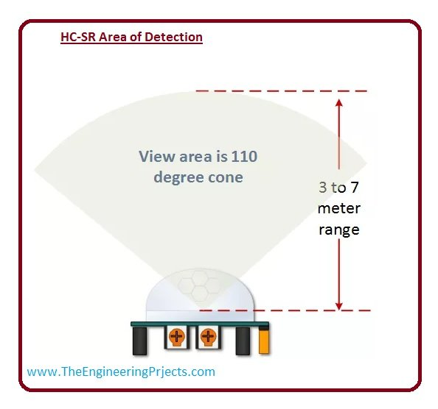
\includegraphics[scale = 0.5]{IR_CONE.png}}
    \caption{Cône de détection du capteur IR}
    \label{fig8}
\end{figure} 

\section{Conclusion}
Nous avons réussi à établir les fondations d'un système de contrôle d'illumnination de trottoir sélectif basé sur la vitesse et le poids d'un objet à sens unique.
Les pronlèmes de détections proviennet surtout du chevauchage du cône de portée des capteurs Infrarouge cosé par leur proximité, ce qui réduit l'efficaité de leur implémentation à l'échelle
de test présente. Le tableau de bord synchronisé avec la matrice de décision affiche bien l'état du système mais la continuité de la mise à jour du document json doit faire l'effet d'un suivi temporel pyroélectriques
afin d'éviter les retards et une mise à jour effective de l'état du système sur le tableau de bord. Plus de dévellopement est nécessaire afin d'aboutir  à un format final.
\section*{Reconnaissance}

Nous voudrion remercier le professeur Mahmoud Youssef pour l'opportunité d'accomplir ce projet ainsi
que l'assistant à l'enseignement Mohammed Yassine Bouhamidi pour son aide et orientation dans l'implémentation des technologie de communication en ligne.



\begin{thebibliography}{00}
\bibitem{b1} “La Pollution Lumineuse.” Les Avantures De Rafale, Environnement Et Lutte Contre Les Changements Climatiques, Québec, https://www.environnement.gouv.qc.ca/jeunesse/chronique/2005/0503-causes.htm. 
\bibitem{b2} Zappi, Piero, et al. “Tracking Motion Direction and Distance with Pyroelectric IR Sensors.” IEEE Sensors Journal, vol. 10, no. 9, Sept. 2010, pp. 1486–1494., https://doi.org/10.1109/jsen.2009.2039792.
\bibitem{b3} "4-Wire Load Cell (1/5/10/20/200kg) with HX711 and Arduino - Circuit Journal". https://circuitjournal.com/four-wire-load-cell-with-HX711 (consulté le 8 octobre 2022).
\bibitem{b4} “How HC-SR501 PIR Sensor Works and How To Interface It With Arduino,” Last Minute Engineers, Jul. 03, 2018. https://lastminuteengineers.com/pir-sensor-arduino-tutorial/ (accessed Dec. 07, 2022).
\bibitem{b5} "Infrared Sensors Overview: Types, Functioning and Use Cases | Kisi". https://www.getkisi.com/guides/infrared-sensors (consulté le 10 octobre 2022).
\bibitem{b6} $https://github.com/Driss-001/ELG4539_trottoir$
\end{thebibliography}
\vspace{12pt}
\color{red}
IEEE conference templates contain guidance text for composing and formatting conference papers. Please ensure that all template text is removed from your conference paper prior to submission to the conference. Failure to remove the template text from your paper may result in your paper not being published.

\end{document}
